\documentclass[8pt]{beamer}
\usetheme{Madrid}
\usefonttheme{serif}

\usepackage{fontspec}
% надёжный шрифт с кириллицей (работает в Overleaf)
\setmainfont{Libertinus Serif}[Ligatures=TeX]
\setsansfont{Libertinus Sans}[Ligatures=TeX]
\newfontfamily\cyrillicfont{Libertinus Serif}
\newfontfamily\cyrillicfontsf{Libertinus Sans}
\usepackage{polyglossia}
\setmainlanguage{russian}
\setotherlanguage{english}

\usepackage{amsmath}
\usepackage{amsfonts}
\usepackage{amssymb}
\usepackage{graphicx}
\usepackage{microtype}

\usepackage{tabularx}
\usepackage{booktabs}

\usepackage{xcolor}
\usepackage{pifont}
\usepackage{tikz}
\newcommand{\plus}{\tikz[baseline=(X.base)] \node[fill=green!65!black, rounded corners=2pt, inner sep=2pt] (X) {\color{white}\ding{51}};}
\newcommand{\minus}{\tikz[baseline=(X.base)] \node[fill=red!70!black,   rounded corners=2pt, inner sep=2pt] (X) {\color{white}\ding{55}};}

\DeclareMathOperator{\sen}{sen}
% \DeclareMathOperator{\tg}{tg}

\setbeamertemplate{caption}[numbered]

% --- Информация о презентации ---
\author[Автор]{Чиняев Владимир Николаевич}
\title{Практические аспекты орбитальных операций \\ Цикл орбитальных операций}
\newcommand{\coursename}{Введение в маневрирование КА}
\setbeamertemplate{navigation symbols}{} 
\institute[]{Московский физико технический институт} 
\date{2 декабря 2025 г.} 

\bibliographystyle{apalike}

% --- Кастомная нижняя синяя полоска: курс слева, номер слайда справа ---
\setbeamertemplate{footline}{
  \leavevmode%
  \begin{beamercolorbox}[wd=\paperwidth,ht=2ex,dp=1ex]{palette primary}
    \hspace{0.4cm}\usebeamerfont{footline}\coursename\hfill\usebeamerfont{footline}\insertframenumber\hspace{0.4cm}
  \end{beamercolorbox}%
}

% Чтобы убрать лишние отступы в footer-шрифте (опционально)
\setbeamerfont{footline}{size=\small}

\begin{document}

\begin{frame}
\titlepage
\end{frame}

\begin{frame}{Цикл орбитальных операций}
\begin{center}
    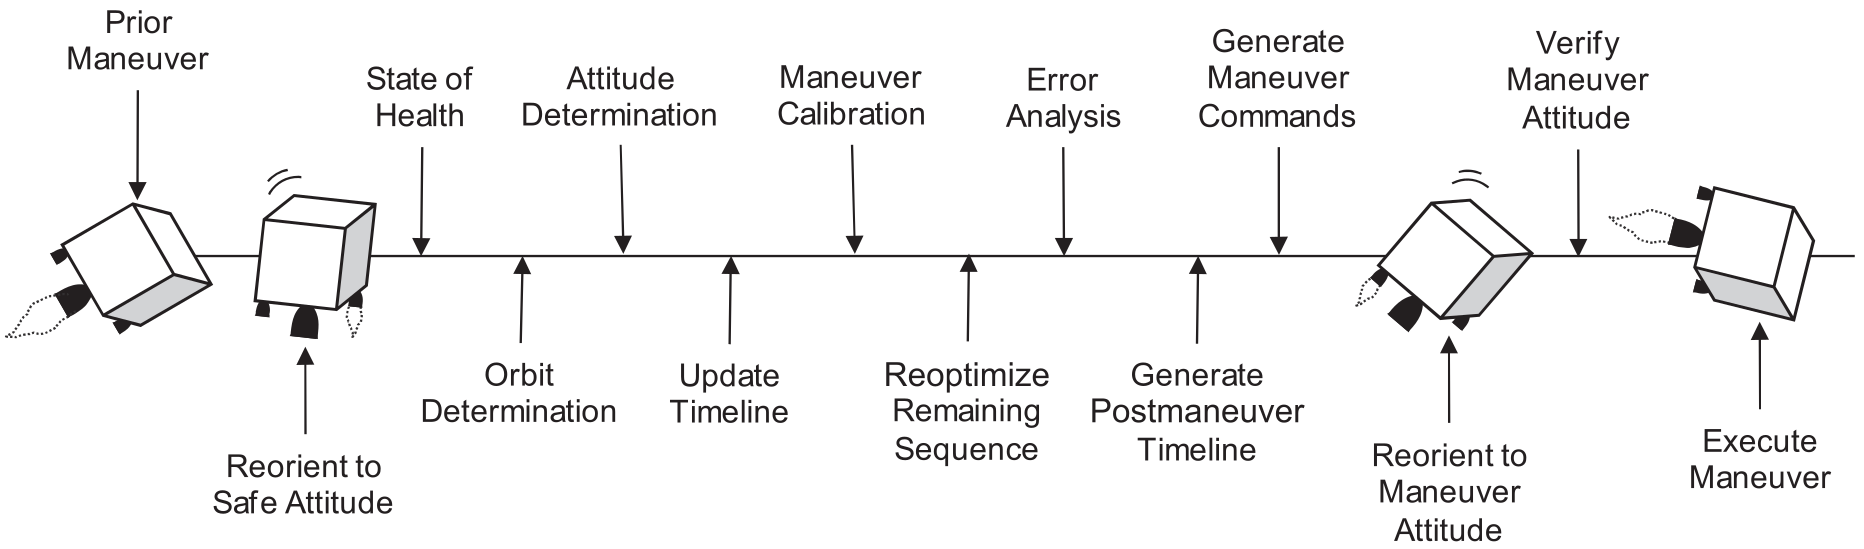
\includegraphics[height=0.35\textheight,keepaspectratio]{images/10/cycle.png}
\end{center}
Типичная последовательность орбитального перехода может быть разделена на несколько этапов, границами которых служат отделение от ракеты-носителя, выполнение манёвра орбитальной коррекции или начало штатной эксплуатации. \\
\smallskip
Деятельность специалистов по баллистике внутри каждого такого этапа, как правило, весьма однотипна. Например, после орбитального манёвра (или после отделения от носителя) специалист выполняет определение орбиты и ориентации. На основе обновлённых данных планируется следующий манёвр и формируются соответствующие команды для КА. Таким образом, между основными событиями баллистик обычно выполняет один и тот же набор операций.
\end{frame}

\begin{frame}{1. Оценка состояния космического аппарата}
\textbf{Когда выполняется:}
\begin{itemize}
    \item После отделения от ракеты-носителя;
    \item После каждого манёвра.
\end{itemize}
\textbf{Цель:} проверить состояние КА по телеметрии и убедиться, что все параметры находятся в пределах ожидаемых значений. \\
\smallskip
\textbf{Проверяются основные данные:}
\begin{itemize}
    \item Температуры и давления;
    \item Углы на Солнце;
    \item Скорости вращения;
    \item Суммарное время работы ДУ;
    \item Оценки орбиты и ориентации (если формируются на борту).
\end{itemize}
\textbf{Если данные штатные}: операции продолжаются по плану. \\
\textbf{Если есть отклонения}: проводится анализ причин. \\
\smallskip
Основную работу выполняют специалисты по подсистемам: системы управления, ДУ, энергоснабжение, терморегулирование, полезная нагрузка и тд. Специалист по баллистике анализирует лишь ограниченный набор данных.
\end{frame}

\begin{frame}{2. Определение орбиты}
После подтверждения исправности КА выполняется определение орбитального состояния по доступным измерениям. Существуют два возможных варианта:
\begin{itemize}
    \item \textbf{Определение орбиты на борту} \\
    Возможно, если на борту есть GPS приёмник и возможности КА позволяют провести соответствующие вычисления. \plus\ Быстрый способ определения орбиты.

    \item \textbf{Определение орбиты на Земле} \\
    Выполняется с помощью дальномерных измерений с телескопов. \minus\ Аппарат должен пройти значительную часть орбиты. \minus\ Обработка измерений требует времени.
\end{itemize}
\textbf{Важно:} определение орбиты происходит лишь по новым данным, полученным после манёвра или отделения от ракеты носителя, для получения наилучшей оценки орбитального состояния.
\end{frame}

\begin{frame}{3. Передача обновлённого орбитального состояния}
После определения орбиты, обновлённое орбитальное состояние передаётся на все наземные станции, поддерживающие миссию. \\
\smallskip
\textbf{Зачем это нужно:}
\begin{itemize}
    \item Послеманевровая оценка орбиты точнее предманеврового предсказания;
    \item Более точное состояние повышает вероятность успешного захвата КА на последующих сеансах связи.
    \item Без обновления увеличивается риск потери КА станцией. Ведь если манёвр сильно отклонился от прогноза, то времена контактов с наземными станциями могут существенно измениться.
\end{itemize}
\end{frame}

\begin{frame}{4. Определение ориентации}
\textbf{Зачем выполняется:} даже если ориентация манёвра была задана фиксированной в инерциальном направлении, в реальности ориентация КА претерпевает изменения. \\
\textbf{Причины изменения ориентации:}
\begin{itemize}
    \item Импульсы при включении и выключении двигателей вызывают небольшие возмущения ориентации;
    \item Остаточные несбалансированные моменты двигателей ориентации;
    \item Крупные выдвижные элементы КА подвержены воздействию внешних моментов.
\end{itemize}
\textbf{Способы определения ориентации:}
\begin{itemize}
    \item \textbf{Ориентация определяется на борту}
    \begin{itemize}
        \item Современные КА используют звёздные датчики или датчики Земли;
        \item Решение об ориентации вычисляется на борту и передаётся по телеметрии;
        \item Баллистик лишь проверяет, что послеманевровая ориентация в пределах нормы.
    \end{itemize}

    \item \textbf{Ориентация определяется на Земле}
    \begin{itemize}
        \item Передаются сырые измерения, которые обрабатываются наземным ПО;
        \item Часто требуется знание текущего положения КА, поэтому сначала выполняется определение орбиты.
    \end{itemize}
\end{itemize}

Измерения ориентации обычно обрабатываются в рамках \textbf{взвешенной процедуры наименьших квадратов} для получения ориентации, наилучшим образом согласующейся с наблюдениями.
\end{frame}

\begin{frame}{5. Обновление бортовой оценки состояния}
\begin{itemize}
    \item На борту КА поддерживается текущая оценка орбиты и ориентации;
    \item Со временем точность этой оценки ухудшается. Скорость деградации зависит от конкретного алгоритма, работающего на бортовом процессоре.
\end{itemize}
\textbf{Зачем обновлять:} чтобы восстановить актуальную информацию орбиты и ориентации. Обновление выполняется по последней оценке, вычисленной на Земле. \\
\smallskip
\textbf{Как часто обновлять:}
\begin{itemize}
    \item Интервал определяется предстартовым анализом;
    \item Обычно обновления выполняются раз в день или реже. Это может быть необходимо или нет — в зависимости от времени, прошедшего с последнего обновления, и от предполагаемой точности текущей бортовой оценки.
\end{itemize}
\end{frame}

\begin{frame}{6. Обновление прогноза событий КА}
После получения новой оценки состояния и ориентации КА выполняется прогноз баллистического движения и обновляется прогноз различных событий. \\
\textbf{Что это за события:}
\begin{itemize}
    \item Проходы над наземными станциями;
    \item Интервалы доступности бортовых антенн;
    \item Времена входа/выхода из тени;
    \item Интервалы работы датчиков ориентации (например, доступность датчиков Земли);
    \item Интервалы, связанные с другими аппаратами;
    \item Интервалы радиопомех;
    \item Прочие события: апогей, перигей, переходы узлов.
\end{itemize}

Обновлённый прогноз событий обычно передаётся всем специалистам и организациям, участвующим в обеспечении миссии, чтобы вся команда работала с актуальной информацией.
\end{frame}

\begin{frame}{7. Оценка возможных сближений с другими КО}
\textbf{Анализ опасных сближений:}
\begin{itemize}
    \item Используя последнюю оценку состояния КА, осуществляется баллистический прогноз;
    \item Состояние сравнивается с каталогом КО;
    \item Для каждого опасного сближения оценивается риск столкновения.
\end{itemize}
Если риск столкновения выше установленного порога, то оператор может выбрать:
\begin{itemize}
    \item Ничего не предпринимать;
    \item Дождаться получения дополнительных данных для уточнения динамики вероятности столкновения (снижается ли риск);
    \item Спланировать манёвр уклонения.
\end{itemize}
Желательно заранее определить и задокументировать план действий при опасных сближениях ещё до запуска.
\end{frame}

\begin{frame}{8. Реконструкция, оценка и калибровка манёвров}
\textbf{Цель:} определить фактические параметры выполненного манёвра и откалибровать модель тяги. \\
\textbf{Выполняется:}
\begin{itemize}
    \item Реконструкция манёвра с помощью процедуры дифференциальной коррекции, что позволяет получить манёвр, наилучшим образом согласующийся с наблюдаемыми орбитальными данными.
    \item Определение фактических величины и направления $\Delta V$.
\end{itemize}
\textbf{Анализируются:}
\begin{itemize}
    \item Ошибки наведения;
    \item Ошибки величины тяги.
\end{itemize}
После реконструкции манёвра стандартной практикой является \textbf{оценка} его качества через отношение приложенного $\Delta V$ к запланированному. Это отношение используется для \textbf{калибровки} модели двигательной установки, чтобы прогнозы будущих манёвров были точнее.
\end{frame}

\begin{frame}{9. Прогнозирование работы двигательной установки}
После калибровки модели ДУ используют обновлённую модель для получения необходимых прогнозов
\begin{itemize}
    \item тяги,
    \item удельного импульса,
    \item расхода рабочего тела
\end{itemize}
при планировании следующих манёвров. \\
\smallskip
Модели ДУ часто требуются значения температур и давлений на момент выполнения манёвра. Поэтому инженер по ДУ подготавливает эти данные на моменты будущих манёвров. \\
\smallskip
\textbf{Результатом этапа может быть:}
\begin{itemize}
    \item Временной профиль тяги,
    \item Временной профиль удельного импульса,
    \item Постоянные значения тяги и удельного импульса (для простейших моделей ДУ).
\end{itemize}
\end{frame}

\begin{frame}{10. Оптимизация оставшейся последовательности манёвров}
После получения обновлённых параметров ДУ, орбиты и ориентации КА, выполняется повторная оптимизация оставшихся манёвров. \\
\smallskip
\textbf{Причины:}
\begin{itemize}
    \item Манёвры никогда не выполняются идеально;
    \item Без перепланирования ошибки будут накапливаться.
\end{itemize}
Баллистики используют специальное ПО, которое учитывает:
\begin{itemize}
    \item Орбиту и ориентацию КА;
    \item Массу и геометрические характеристики КА (моменты инерции, расположение двигателей);
    \item Данные о ДУ (тяга, удельный импульс, расход рабочего тела);
    \item Параметры манёвров (число манёвров, веса манёвров, структура витков);
    \item Целевые параметры конечной орбиты и тд.
\end{itemize}
\textbf{Наиболее важные данные} — параметры ближайшего манёвра: время начала, величина $\Delta V$, направление $\Delta V$.
\end{frame}

\begin{frame}{11. Анализ ошибок}
\textbf{Цель:} проверить устойчивость нового плана манёвров к типичным статистическим ошибкам. \\
\smallskip
\textbf{Какие ошибки учитываются:}
\begin{itemize}
    \item Ошибки вывода КА ракетой-носителем;
    \item Ошибки наведения;
    \item Ошибки работы ДУ;
    \item Опоздание манёвра;
    \item Пропуск манёвра и тд.
\end{itemize}
Если в текущем плане выявляется недостаток, его необходимо изменить и повторно оптимизировать на шаге 10, чтобы устранить проблему.
\end{frame}

\begin{frame}{12. Формирование команд для КА}
Данные, необходимые для задания протяжённых манёвров: время начала, длительность манёвра, ориентация КА. Данные о манёврах должны быть преобразованы в формат, который понимает бортовая система:
\begin{itemize}
    \item \textbf{Время начала манёвра может задаваться как:}
    \begin{itemize}
        \item календарная дата;
        \item секунды от J2000;
        \item GPS-секунды;
        \item секунды от начала суток;
        \item время обратного отсчёта от момента передачи команды.
    \end{itemize}

    \item \textbf{Команды переориентации могут требовать:}
    \begin{itemize}
        \item начальных и конечных значений прямого восхождения и склонения;
        \item начальных и конечных кватернионов;
        \item фазового угла, длительности импульсов, числа импульсов (для переориентации с помощью ДУ).
    \end{itemize}
\end{itemize}
\textbf{Параметры манёвра должны быть преобразованы в набор конкретных команд именно для данного КА.} \\
\smallskip
Помимо «основных» команд обычно требуется отправить и множество дополнительных. Часто формируются команды защиты на случай, если манёвр пойдёт не по плану. Например
\begin{itemize}
    \item Ограничения по углу на Солнце с аварийным прерыванием манёвра при выходе за предел.
    \item Резервный таймер, чуть превышающий номинальную длительность манёвра, который закрывает клапаны двигателей.
    \item Ограничения по скорости вращения; либо по суммарному времени работы двигателей / числу импульсов.
    \item Команды на открытие запорных клапанов в магистралях подачи рабочего тела.
\end{itemize}
\end{frame}

\begin{frame}{13. Обновление прогноза событий после манёвра}
\textbf{Что было сделано ранее (шаг 6):} сформирована последовательность событий по наблюдаемому состоянию после предыдущего манёвра. \\
\smallskip
\textbf{Что требуется сейчас:} 
\begin{itemize}
    \item Учесть предстоящий манёвр и его расчётное влияние на орбиту и ориентацию.
    \item Сформировать прогноз событий после нового манёвра.
\end{itemize}
\textbf{Зачем это нужно:}
\begin{itemize}
    \item Чтобы заранее спланировать действия команды после предстоящего импульса.
\end{itemize}
Обновлённые послеманевровые прогнозы генерируются по имеющимся данным и распространяются среди всех участников команды.
\end{frame}

\begin{frame}{14. Формирование плана действий на случай пропуска манёвра}
\textbf{Что сделано ранее:} на шаге 11 проверено, что при пропуске манёвра существует выполнимый альтернативный план. \\
\smallskip
\textbf{На этом этапе подготавливается полный комплект материалов для резервного плана:}
\begin{itemize}
    \item результаты анализов ошибок (ошибка наведения, поздний старт, пропуск манёвра и др.);
    \item пакет команд для КА;
    \item обновлённый график событий.
\end{itemize}
\textbf{Зачем это нужно:} для того, чтобы обеспечить возможность немедленного перехода на резервный план, если предстоящий манёвр будет пропущен. \\
\smallskip
\textbf{Важно, что такой анализ проводится лишь после подготовки номинального плана.} \\
\smallskip 
Для других возможных ситуаций (опоздание манёвра, ошибки наведения, прерывание манёвра) такой анализ не готовится заранее, поскольку невозможно предсказать конкретный момент задержки, величину ошибки или точку прерывания манёвра.
\end{frame}

\begin{frame}{15. Выполнение манёвра в имитационной модели КА}
Часто в миссиях существует полный программный клон реального КА, который может точно смоделировать различные режимы работы КА. \\
\smallskip
\textbf{Зачем это нужно:}
\begin{itemize}
    \item Проверить корректность сформированного пакета команд.
    \item Убедиться, что манёвр отрабатывается так, как запланировано.
\end{itemize}
\end{frame}

\begin{frame}{16. Утверждение манёвра}
На заключительном этапе проверки во многих миссиях требуется проведение совещания по утверждению манёвра, прежде чем любые команды будут переданы на космический аппарат. На таком совещании ответственные инженеры (представители всех подсистем — системы управления, баллистики, двигательной установки и др.) представляют руководству программы (а иногда и заказчику аппарата) план предстоящего манёвра. \\
\smallskip
\textbf{Что представляется:}
\begin{itemize}
    \item Цель манёвра;
    \item Основные параметры: длительность, расход/остаток топлива, ориентация;
    \item Пакет команд, планируемый к загрузке;
    \item Состояние подсистем и ожидаемое поведение во время манёвра;
    \item Результаты проверки на имитационной модели;
    \item Прогнозируемое послеманевровое состояние;
    \item Резервные сценарии.
\end{itemize}
Когда все вопросы закрыты, руководство даёт разрешение на выполнение манёвра.
\end{frame}

\begin{frame}{17. Загрузка команд на борт КА}
Во время сеанса связи с наземной станцией, предшествующего времени манёвра, на борт передаются соответствующие команды. \\
\smallskip
\textbf{Что выполняется:}
\begin{itemize}
    \item Передача пакета команд на борт космического аппарата;
    \item Получение по телеметрии подтверждения принятых команд.
\end{itemize}
Это относится ко всем типам манёвров: орбитальным коррекциям, переориентациям и тд.
\end{frame}

\begin{frame}{18. Контроль выполнения манёвра}
После передачи команд на КА команда управления отслеживает телеметрию во время выполнения манёвра (если манёвр выполняется в зоне видимости). Если какой-либо параметр выходит за ожидаемые пределы (углы на Солнце, температуры и т. д.), это фиксируется как проблема, и \textbf{принимается решение о продолжении или прекращении манёвра}.
\end{frame}

\begin{frame}[allowframebreaks]{Источники}
  \begin{thebibliography}{9}

    \bibitem{DiPrinzio}
    DiPrinzio M. Methods of Orbital Maneuvering. – American Institute of Aeronautics and Astronautics, Inc., 2019.
    
  \end{thebibliography}
\end{frame}

\end{document}
